\documentclass[12pt,a4paper]{article}
\usepackage[utf8]{inputenc}
\usepackage[T1]{fontenc}
\usepackage[spanish,mexico]{babel}
\usepackage[margin=2.5cm]{geometry}
\usepackage{graphicx}
\usepackage{float}
\usepackage{caption}
\usepackage{subcaption}
\usepackage{fancyhdr}
\usepackage{hyperref}
\usepackage{listings}
\usepackage{xcolor}
\usepackage{booktabs}
\usepackage{enumitem}

\pagestyle{fancy}
\fancyhf{}
\fancyhead[L]{Proyecto de Chat TCP}
\fancyhead[R]{Facultad de Ciencias, UNAM}
\fancyfoot[C]{\thepage}

\hypersetup{
    colorlinks=true,
    linkcolor=black,
    urlcolor=blue,
    citecolor=black
}

\title{Proyecto 1: Chat TCP}
\author{Espinosa Meléndez Juan Ernesto}
\date{\today}

\begin{document}
\thispagestyle{empty}
\begin{figure}[H]
    \centering
    \includegraphics[width=4cm]{unam-logo-png_seeklogo-144764.png}
    \hspace{2cm}
    \includegraphics[width=4cm]{FC1.png}
\end{figure}

\vspace{1cm}

\begin{center}

    {\Large \textbf{UNIVERSIDAD NACIONAL AUTÓNOMA DE MÉXICO}}\\[0.5cm]

    {\Large \textbf{FACULTAD DE CIENCIAS}}\\[1.5cm]

    {\LARGE \textbf{Proyecto 1}}\\[0.5cm]

    {\Large \textbf{Chat TCP}}\\[1.5cm]

    \textbf{Alumno:}\\
    Espinosa Meléndez Juan Ernesto\\
    No. de cuenta: 323150066\\[1cm]

    \textbf{Asignatura:}\\
    [Modelado y Programación]\\[0.8cm]

    \textbf{Profesor:}\\
    [Canék Peláez Valdés]\\[1cm]

\end{center}

\newpage

\tableofcontents

\newpage

\section{Introducción}
Este proyecto trata sobre el análisis, modelado y desarrollo de un chat TCP, en donde debíamos investigar como programar un servidor 
y un cliente que se pudieran comunicar entre si. Además, debíamos determinar en que lenguaje se iba a programar, en este caso se realizó
 el servidor en C y el cliente en C++, tomando en cuenta que debíamos enviar y recibir de manera interna mensajes JSON que el usuario no 
 iba a poder ver ni escribir, pero en cambio el servidor si debía lidiar con ellos.\\

Una vez terminadas las bases teníamos un protocolo que se debía cumplir para crear salas privadas y una sala pública, enviar invitaciones 
y aceptarlas, solicitar la lista de usuarios en las respectivas salas, cambiar el estatus e identificarse. Durante las clases se fueron 
dando otras indicaciones que complementaron el protocolo, tales fueron los casos de definir un límite al tamaño de mensajes, ya que solo 
existía un límite en el username que podía utilizar un usuario y un límite en el nombre de las salas privadas.
\\
Este proyecto da por hecho que el programa va a funcionar adecuadamente, ya que se cuentan con las bases necesarias, siendo que lo más 
importante es el análisis, modelado y desarrollo del mismo, sin embargo como se verá más adelante, hubo distintos problemas a la hora del 
desarrollo y en la cuestión del modelado.

\section{Análisis y modelado}
\subsection{Análisis}
La elección del lenguaje fue algo que no pensé demasiado, ya que, Canek ofreció 1 punto extra si hacíamos el servidor en C y el usuario en 
un lenguaje distinto, así que opté por utilizar C en el servidor y C++ para el usuario, no solo por el punto extra que ofreció Canek, sino 
que también contaba con libros para aprender a programar en C y C++, implementar algoritmos en C y de programación estructurada en C; con 
esto como base pensé que sería sencillo utilizar estos 2 lenguajes dado que contaba con bibliografía a la mano que me podía ser de utilidad 
y además podía aspirar a 2 puntos extra.
\\
Antes de comenzar, busqué distintos tutoriales para saber como se hacía un servidor, adicionalmente leí como funcionaban los sockets porque 
esto era muy importante para el proyecto y era algo de lo que no tenía ni idea de como implementarlo. Afortunadamente encontré un par de 
tutoriales que me fueron de gran utilidad al comienzo.
\\
Mi idea al comienzo era realizar una interfaz y que el programa sería parecido al messenger viejito que tenía zumbidos, visualmente me 
podía dar una idea, sin embargo en la cuestión del servidor lo único que tenía claro era lo que había podido observar en los tutoriales, 
adicionalmente lo único que sabía de C y C++ era lo que había podido leer en la primera semana.
\\
Lo que pensé para el orden de como desarrollar el proyecto fue: comenzar el servidor hasta que aceptara conexiones y utilizar un usuario de 
prueba que me permitiera asegurarme que el servidor funcionaba. En este punto pude haber hecho tests para no hacerlo manualmente pero la 
verdad no tenía idea de como hacerlas y cada vez me quedaba menos tiempo para la fecha de entrega y no tenía nada en mi repositorio más que 
el archivo de prueba. Posteriormente traté te hacer que el servidor fuera estable, guardara los clientes en un diccionario, funcionará la 
lista de usuarios conectados y pudieras cambiar tu estatus, para que una vez terminara con esto fuera de lleno con todo lo que abarcaba el 
protocolo respecto a salas y enviar mensajes.\\
El cliente en algún punto tenía que crearlo, pero lo pospuse lo más que pude ya que no había investigado tantas cosas de C++ como lo hice 
con C, cuando el cliente de prueba me dejo de ser útil lo deseche y comencé con el desarrollo de uno propio que pudiera cumplir con todo 
lo que el protocolo requería.
\\
Una vez que ya había comenzado, los tutoriales comenzaron a ser escasos y me guié por repositorios que habían hecho un proyecto similar o 
igual al que me pedían, sin embargo, algunos no me eran completamente de utilidad, ya que algunos limitaban la cantidad de usuarios, no 
usaban JSON o estaban hechos para windows. Por tanto los use más como una guía de lo siguiente que debía hacer, lo bueno es que en el caso 
del cliente al haber escogido C++ contaba con referencias mucho más útiles que para guiarme en el desarrollo del servidor en C.
\subsection{Modelado}
Traté de programar siguiendo algún patrón de diseño, claro que el que tuve más claro fue el del cliente con MVC, sin embargo para el caso 
del servidor la cosa se me complicó bastante, ya que al comienzo simplemente seguí los tutoriales y creí que me sería más fácil identificar 
cual utilizar en cada caso. Sin embargo, terminé optando por hacer todo el programa de golpe y separarlo adecuadamente cuando estuviera 
terminado. \\
Entiendo que es una mala práctica y si bien llegué a separar unas cosas que me parecieron más sencillas de identificar porque no me convenía 
dejarlas juntas, en su momento creí que el loop infinito dentro del servidor sería pequeño y que solo agregaría lo indispensable. En la 
práctica terminé añadiendo todo porque cuando me dí cuenta que lo tuve que haber separado desde un inicio ya era un poco tardé y prioricé 
terminar todo antes de tratar de seguir un patrón que me facilitara las cosas.
\\
El tener todo el servidor en 2 clases hizo que eventualmente me perdiera con facilidad y se complicará el modificar las cosas cuando algo se 
rompía o no funcionaba como lo había pensado, practicamente utilizaba el ctrl + f en todo momento. Lo único bueno es que desde el comienzo 
fui dejando comentarios que me permitían saber que hacía cada parte, además de que los nombres de las variables los hice lo más explícitos 
que podía pero tratando de que fueran cortos porque me terminaría hartando de escribir un nombre largo y poco eficaz.
\\
Eventualmente realicé distintas refactorizaciones para ayudarme a encontrar con mayor facilidad las cosas, además de corregir partes que 
durante las clases alguien que había hecho algo similar recibía la indicación por parte de Canek de que estaba mal hecho, así que 
aprovechaba para cambiarlo yo también antes de que fuera demasiado tarde.\\
\section{Descripción general del sistema}

\subsection{Arquitectura cliente/servidor}

\begin{figure}[H]
    \centering
    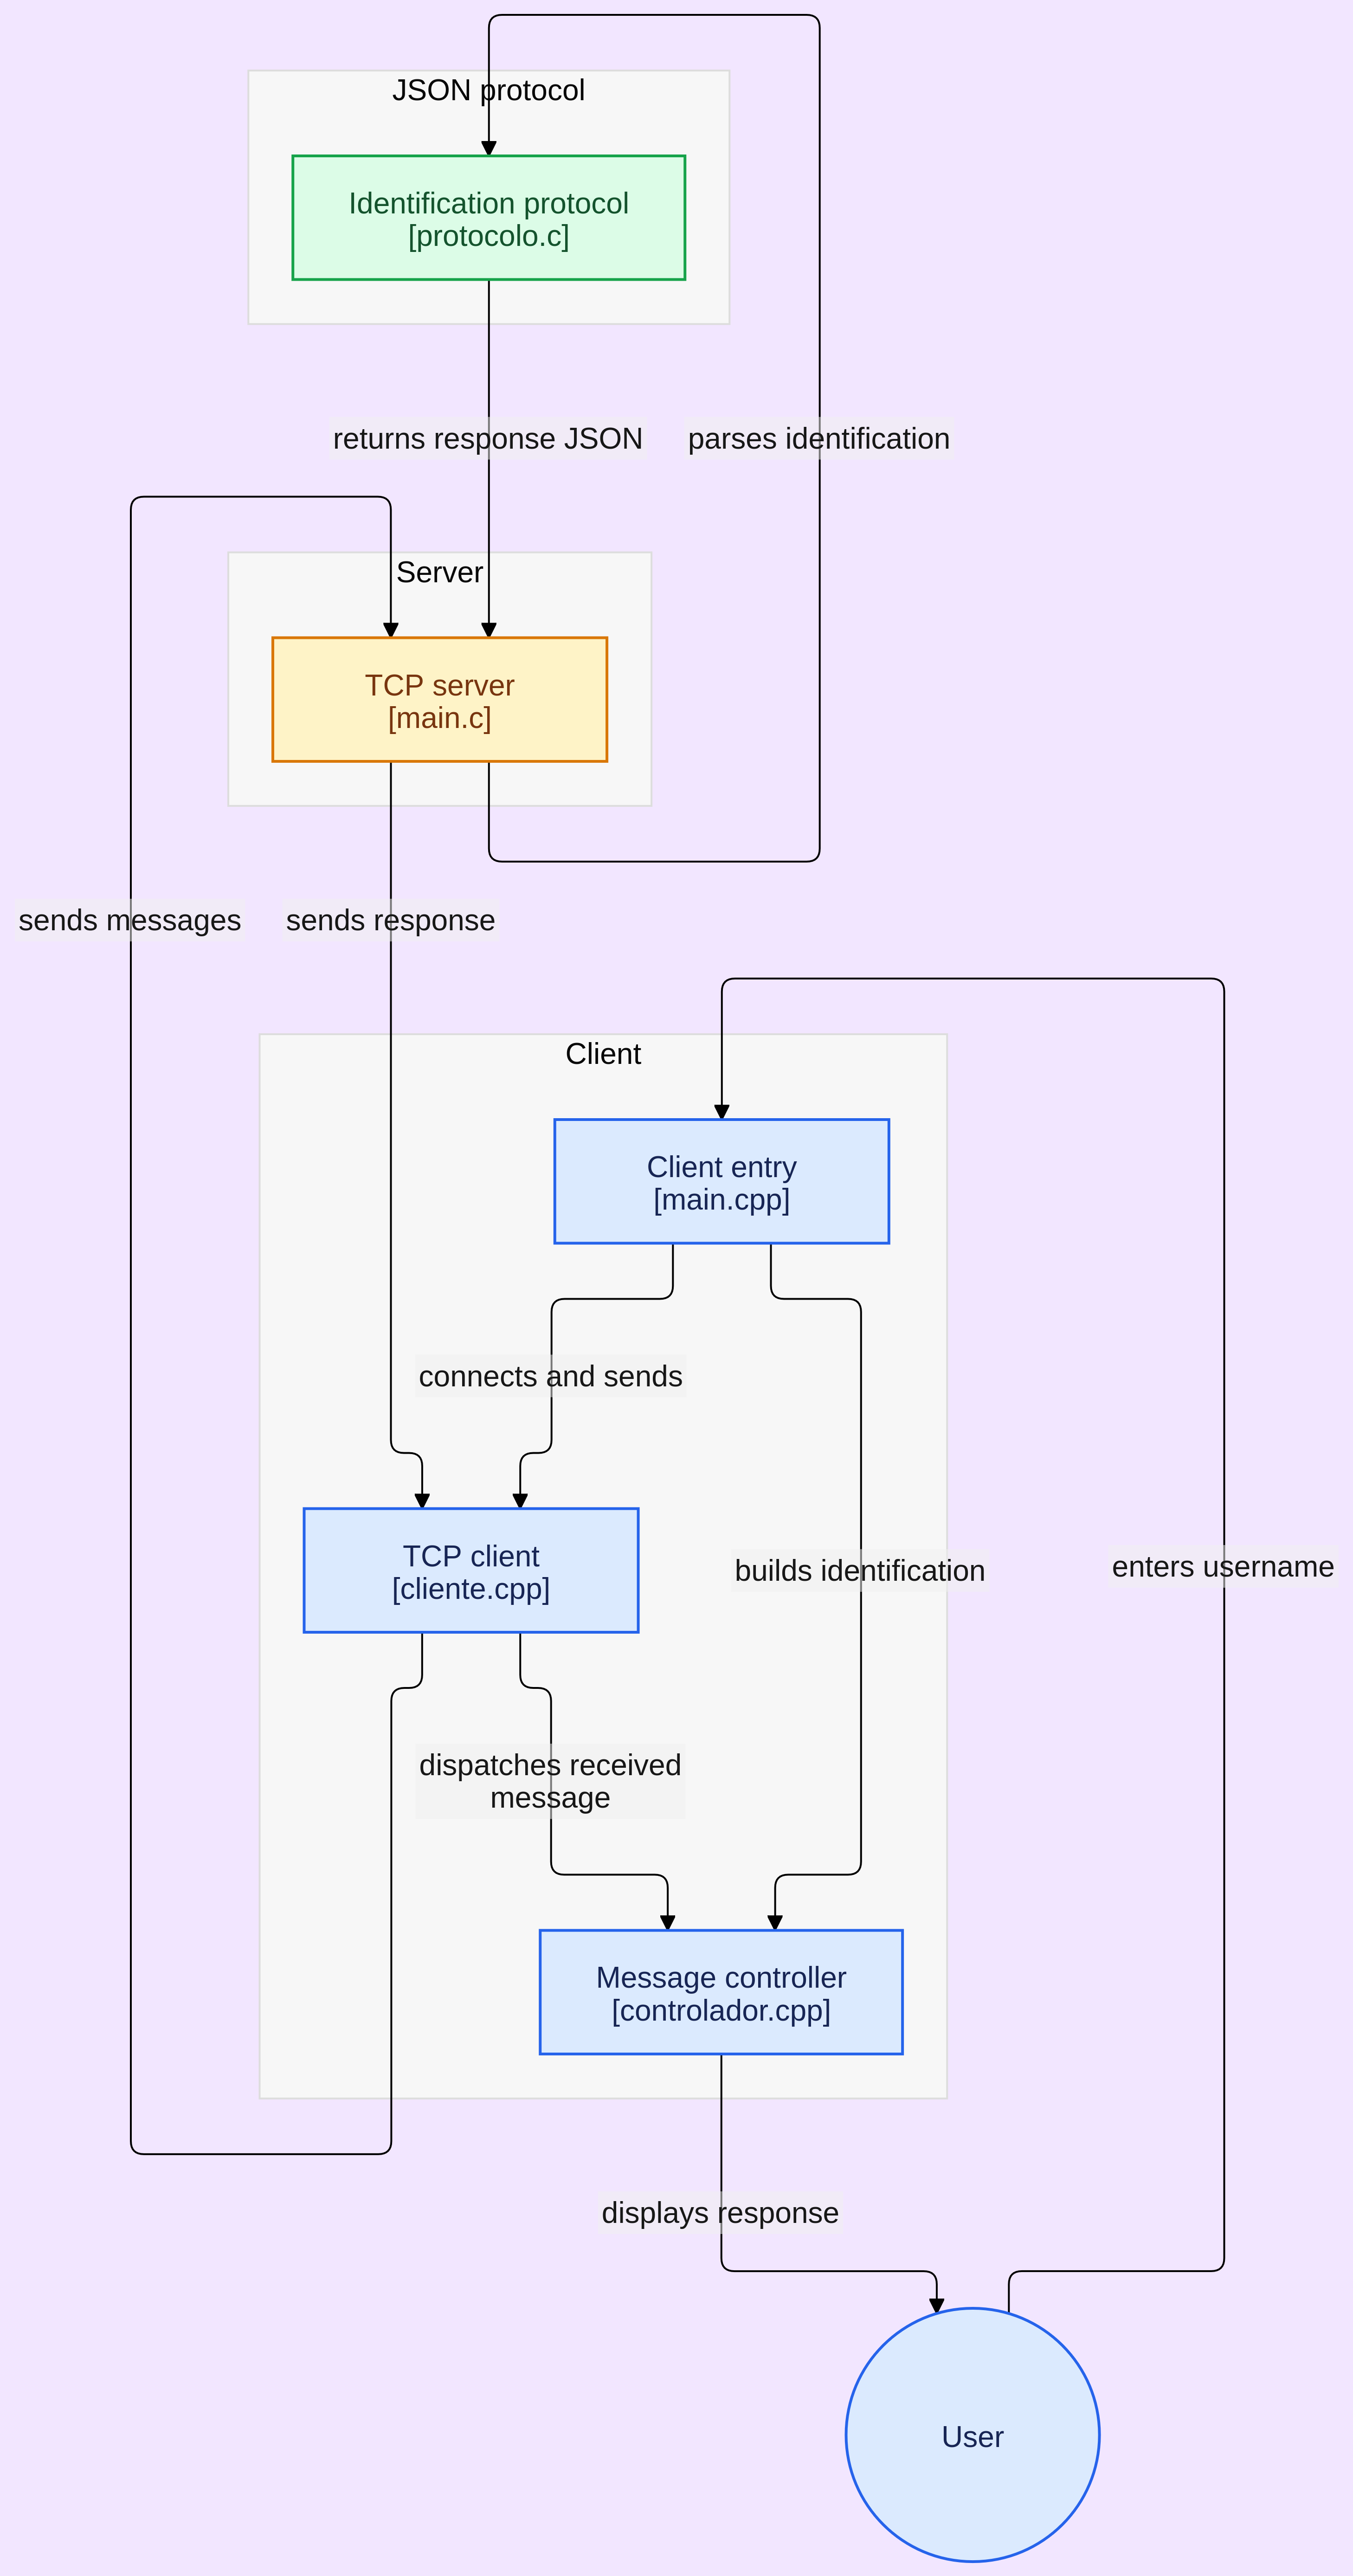
\includegraphics[width=0.55\textwidth]{diagram.png}
    \label{fig:arquitectura}
\end{figure}

\section{Protocolo de comunicación}
\subsection{Operaciones del protocolo}
\begin{itemize}
    \item IDENTIFY
    \item STATUS
    \item USERS
    \item TEXT
    \item PUBLIC\_TEXT
    \item NEW\_ROOM
    \item INVITE
    \item JOIN\_ROOM
    \item ROOM\_USERS
    \item ROOM\_TEXT
    \item LEAVE\_ROOM
    \item DISCONNECT
\end{itemize}
\begin{table}[H]
    \centering
    \begin{tabular}{@{}ll@{}}
        \toprule
        \textbf{Operación} & \textbf{Descripción} \\
        \midrule
        IDENTIFY & Identifica al usuario ante el servidor con un nombre. \\
        STATUS & Cambia el estado del usuario (\texttt{ACTIVE}, \texttt{AWAY} o \texttt{BUSY}). \\
        USERS & Solicita la lista de usuarios conectados y su estado. \\
        TEXT & Envía un mensaje privado a otro usuario. \\
        PUBLIC\_TEXT & Envía un mensaje a todos los usuarios conectados. \\
        NEW\_ROOM & Crea una nueva sala, de la que el creador es el primer miembro. \\
        INVITE & Invita a uno o más usuarios a una sala en la que ya se es miembro. \\
        JOIN\_ROOM & Une al usuario a una sala a la que fue invitado. \\
        ROOM\_USERS & Solicita la lista de usuarios de una sala a la que se pertenece. \\
        ROOM\_TEXT & Envía un mensaje a todos los miembros de una sala. \\
        LEAVE\_ROOM & Abandona una sala de la que se es miembro. \\
        DISCONNECT & Se desconecta del chat y abandona todas sus salas. \\
        \bottomrule
    \end{tabular}
    \label{tab:operaciones}
\end{table}
\begin{table}[H]
    \centering
    \begin{tabular}{@{}ll@{}}
        \toprule
        \textbf{Mensaje} & \textbf{Descripción} \\
        \midrule
        NEW\_USER & Un nuevo usuario se identificó en el chat. \\
        NEW\_STATUS & Un usuario cambió su estado. \\
        USER\_LIST & Respuesta a \texttt{USERS}. \\
        TEXT\_FROM & Mensaje privado recibido de otro usuario. \\
        PUBLIC\_TEXT\_FROM & Mensaje público recibido de otro usuario. \\
        INVITATION & Invitación recibida a una sala. \\
        JOINED\_ROOM & Un usuario se unió a una sala. \\
        ROOM\_USER\_LIST & Respuesta a \texttt{ROOM\_USERS}. \\
        ROOM\_TEXT\_FROM & Mensaje recibido dentro de una sala. \\
        LEFT\_ROOM & Un usuario abandonó una sala. \\
        DISCONNECTED & Un usuario se desconectó del chat. \\
        RESPONSE & Resultado de una operación solicitada (éxito o error). \\
        \bottomrule
    \end{tabular}
    \label{tab:notificaciones}
\end{table}

\section{Implementación del servidor}
\subsection{Creación del socket}
El servidor main.c crea un socket TCP con socket(AF\_INET,
SOCK\_STREAM, 0), habilita la opción SO\_REUSEADDR para poder
reiniciarlo sin esperar a que el sistema libere el puerto, lo asocia a
INADDR\_ANY en el puerto configurado con bind() y finalmente
llama a listen() para empezar a aceptar conexiones entrantes.

\subsection{Manejo de múltiples clientes}
El servidor atiende a todos los clientes conectados dentro de un único hilo,
usando poll() sobre un arreglo de struct pollfd. A
diferencia de select(), que trabaja con un fd\_set de tamaño
fijo, poll() recibe un arreglo cuyo tamaño se decide en tiempo
de ejecución. El arreglo de pollfd y el arreglo paralelo de punteros
a struct cliente se reservan dinámicamente y duplican su capacidad
con realloc() cada vez que se alcanza el límite actual, de modo que
el número de clientes conectados simultáneamente solo está limitado por la
memoria disponible.

\subsection{Estructura del cliente}
Cada conexión se representa con una struct cliente, definida en
cliente, que guarda el descriptor del socket, un buffer de lectura
de tamaño variable junto con los bytes actualmente ocupados en él, el nombre
de usuario, si ya se identificó y su estado (ACTIVE, AWAY o
BUSY). Su creación y destrucción se centralizan en
crear\_cliente() y destruir\_cliente() 

\subsection{Gestión de usuarios}
Los usuarios identificados se guardan en un diccionario de usuarios 
que asocia cada nombre de usuario con el puntero a su
struct cliente. Al procesar IDENTIFY se verifica con
g\_hash\_table\_contains() que el nombre no esté en uso; si ya
existe, se responde USER\_ALREADY\_EXISTS y se desconecta al
cliente, y si no, se inserta en la tabla y se notifica a los demás usuarios
identificados con NEW\_USER.

\subsection{Gestión de salas}
Cada sala se representa con una struct sala con su
nombre y dos diccionarios: una de miembros y otra de invitados
pendientes de unirse. Las salas mismas se guardan en un segundo
diccionario global, por nombre de sala. Las
funciones de sala.c:sala\_agregar\_invitado, sala\_unir\_miembro,
sala\_es\_miembro, sala\_es\_invitado, sala\_eliminar\_miembro,
sala\_sin\_miembros. Encapsulan estas dos tablas para que el resto del 
servidor no tenga que manipularlas directamente. Cuando una sala se queda
sin miembros, se elimina de la tabla global y su nombre vuelve a estar
disponible para NEW\_ROOM.

\subsection{Manejo de mensajes}
Los mensajes ya extraídos del buffer del cliente se despachan mediante el
patrón Command implementado en comandos.c.


\section{Implementación del cliente}

\subsection{Programa principal}

\subsection{Controlador}

\subsection{Comunicación TCP}

\subsection{Recepción de mensajes}

\section{Refactorización y patrones de diseño}

\subsection{Factory}

\subsection{Command}

\section{Diagramas UML}

\subsection{Diagrama de componentes}

\subsection{Diagrama de clases}

\subsection{Diagrama de secuencia}

\section{Problemas encontrados y soluciones}

\subsection{Problema 1}

\subsubsection{Solución}

\subsection{Problema 2}

\subsubsection{Solución}

\section{Conclusiones}

\section{Referencias}

\appendix

\end{document}